% \providecommand{\main}{..} 

\documentclass[../main.tex]{subfiles}
\graphicspath{{\subfix{../figures/}}}
\usepackage{bbm}
% \addbibresource{../bibliography/bibliography.bib} % 

\begin{document}

    \chapter{State of the Art} \label{chap:state_of_the_art}

    \section{Relevant Techniques} \label{sec:relevant_techniques}

    While it is important to consider the design of robust machine learning models from their training phase, and part of this work will discuss techniques to optimize for that goal, our primary concern is to provide a model-agnostic framework for maintaining reliability \textit{after} a model has been already deployed.
    % That is, during the inference phase of deployed models.
    
    To accomplish this, we consider a set of novel techniques proposed in the literature to address the problems related to deploying supervised and semi-supervised machine learning models in real-world scenarios. The following section describes these techniques and their relevance to the problem at hand. 
    
    Note that while the focus is on applying these techniques to healthcare applications, it is easy to show that these methods can be generalized to other domains.

    % \clearpage
    
    % \noindent
    % \textit{"Everything is related to everything else, but near things are more related than distant things."} \cite{tobler_computer_1970}
    % \mbox{}\hfill \textit{- Waldo Tobler (1970)}
    
	
	\subsection{Continual Learning} \label{sec:continual_learning}
	
	 Continual learning refers to the concept of constantly updating a model as new information arrives, allowing them to adapt to changing data \cite{huyen_designing_2022}. This constant change in the data distribution requires models to be updated periodically to maintain their accuracy and relevance, prevent model stagnation and extend their relevance to the application.

     We can consider two frameworks for implementing continual learning in a machine-learning system. We refer to the first as \textit{offline learning}, where the model is updated periodically using a batch of data collected over time. Offline learning can be additionally subdivided into two categories based on how data is monitored prior to updating a model: \textit{passive} and \textit{active} continual learning.

     The model is updated passively when the data is collected over a fixed period of time (e.g., every six months) or after a fixed number of instances have been processed and labeled (e.g., every 1000 new instances). Conversely, the model is updated actively when we update only when the model's performance drops below a certain threshold or when the system detects a significant change in the data distribution \cite{huyen_designing_2022}.

    Online learning is the second framework for implementing continual learning. The difference between online and offline learning is that, with the former, the model is updated as soon as new data arrives, with every new instance - or small batch of instances - being used to update the model. Because this approach tends to be more computationally expensive than offline learning and suffers from well-known problems such as catastrophic forgetting \cite{huyen_designing_2022}, it is often used in conjunction with offline learning to improve the model's performance. 

    Continual learning is well-suited for healthcare applications where data arrives in a stream (e.g., wearable health monitors, electronic medical records, and imaging systems). It is also useful in terms of 



	
    \subsection{Active Learning} \label{sec:active_learning}
 
     Active learning strategies selectively acquire data based on their informativeness or uncertainty to the model. Its value comes from allowing the model to guide its own data acquisition process, thus potentially reducing the need for vast - or unnecessary - amounts of pre-labeled data before a model is trained or updated \cite{huyen_designing_2022, chen_study_2015, figueroa_predicting_2012}. 
     This is particularly important in health applications, as the availability of annotated medical data is often limited due to privacy concerns, expert time constraints, and the complexity of pathological findings.
     
     Active learning enables the development of accurate models using significantly less labeled data, paving the way for more efficient and cost-effective machine-learning platforms. Some of the most common active learning strategies include uncertainty sampling, query by committee, and expected model change. 

    \subsection{Adversarial Learning} \label{sec:adversarial_training}

    Adversarial learning is a technique that aims to make models more robust to adversarial examples. Adversarial examples are inputs intentionally designed to be misclassified by a model. They are created by adding small perturbations to the input data, which are imperceptible to humans but can cause the model to make a wrong prediction. Adversarial examples are a major concern in healthcare applications, as they can mislead models into making incorrect diagnoses, misrepresenting the patient's condition, and leading to incorrect treatment decisions \cite{finlayson_adversarial_2019}.

    \begin{figure}[h]
        % \frame{
        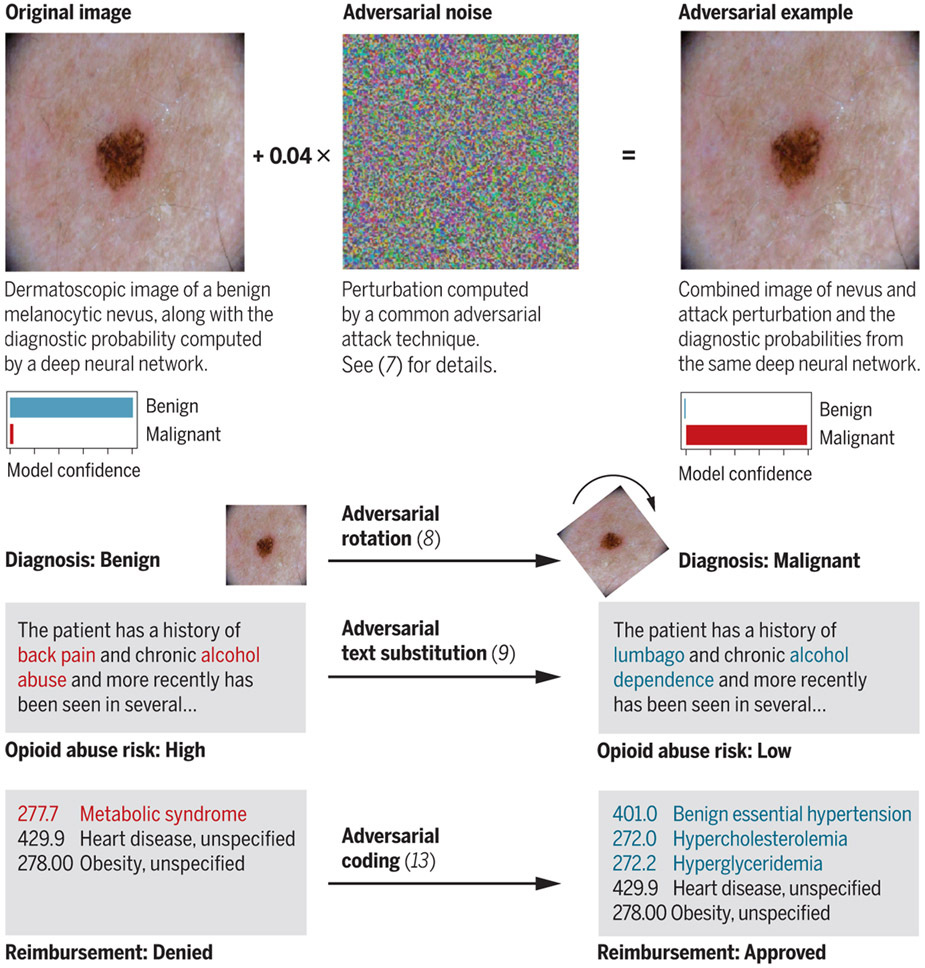
\includegraphics[width=0.65\linewidth]{figures/medical-adversarial-attacks.jpeg}
        \caption{Adversarial examples in medical imaging from Finlayson et al. (2019) \cite{finlayson_adversarial_2019}.}
        % }
    \end{figure}
    % \vspace*{-0.5cm}
    % Adversarial training aims to make models more robust to adversarial examples by training them to be resilient to small perturbations in the input data. This can be achieved by adding a loss term to the training objective that penalizes the model for making incorrect predictions on adversarial examples or by creating a separate adversarial model that is trained to generate adversarial examples that are difficult to detect by the original model and then use those examples for training the original model. 

    
    
    % Adversarial training is a promising technique for improving the robustness of machine-learning models in healthcare applications, as it can be applied to any model architecture and does not require any additional data.

    \subsection{Adaptive Learning with Human Feedback} \label{sec:human_feedback}

    In healthcare applications, feedback from experts is a very important resource, essential for improving the accuracy of the model. This technique aims to explode human feedback as much as possible to obtain model improvements. The goal is to construct policies that adapt the model based on feedback provided by the expert. 
    
    One recent example of this technique is OpenAI's ChatGPT, which used Reinforcement Learning with Human Feedback (RLHF) to instruction fine-tune their GPT-3 language models \cite{christiano_deep_2023,ouyang_training_2022} to align them better with human preferences. RLHF consists of training a reward function that maximizes the probability of the model's predictions matching the expert's feedback. This reward function is then used to train or fine-tune the model using reinforcement learning.

    % For example, a model can be trained to prioritize the detection of a specific disease over others or to provide more accurate predictions for a specific patient.

    % \begin{equation}
    %     \label{eq:human_feedback}
    %     \begin{aligned}
    %         \max_{\theta} & \sum_{i=1}^{n} \sum_{j=1}^{m} \alpha_{ij} \cdot \mathbb{1}(\hat{y}_{ij} = y_{ij}) \\
    %         \text{subject to} & \hat{y}_{ij} = \text{argmax}_{k} \hat{p}_{ijk} \\
    %         & \hat{p}_{ijk} = \sigma(\theta \cdot x_{ij})
    %     \end{aligned}
    % \end{equation}

    % The objective function in Equation \ref{eq:human_feedback} is a weighted sum of the number of times the model and the expert agree on the prediction for each class. $n$ is the number of data points, and $m$ is the number of classes
    %  The weights are determined by the number of times the model and the expert agree on the prediction for the correct class. This objective function is maximized by training the model to prioritize detecting the classes in which the expert has the most confidence.

    \subsection{Meta-Learning} \label{sec:meta_learning} \unsure{Unsure about keeping this section / how relevant it is}

    
    Meta-learning is a technique that aims to improve the performance of machine-learning models by `learning how to learn' a certain task. The way this is formulated is by training a model on a variety of tasks and then using the knowledge gained from those to improve its performance on new tasks, or learn that it faster / more sample-efficiently than if it had been trained only for that task \cite{hospedales_meta-learning_2020}.
    
    Jurgen Schmidhuber first introduced the concept of meta-learning in 1987 \cite{schmidhuber_evolutionary_1987}, and it has since been applied to a wide range of problems, including computer vision, natural language processing, and robotics \cite{hospedales_meta-learning_2020}. Recently, Finn et al. (2017) \cite{finn_model-agnostic_2017} propose a model-agnostic framework for meta-learning that can be applied to any deep-learning architecture and learning task. The framework consists of \dots
    
    The model(s) learn a new set of parameters that can be used to improve its performance on new tasks.

    \todo[inline]{Modify description, add more details, references \dots}

    \subsection{Knowledge Distillation} \label{sec:knowledge_distillation}

    Knowledge distillation is a technique that aims to improve the performance of a model by transferring the knowledge of a larger model (teacher) to a smaller model (student). This is achieved by training the student model to mimic the predictions of the teacher model. The student model is trained on the same data as the teacher model, but it is trained to predict the probabilities of the teacher model's predictions instead of the actual labels. This allows the student model to learn from the teacher model's mistakes and improve its performance on the given task \cite{hinton_distilling_2015}.
    
    \todo[inline]{Modify description, add more details, references \dots}
    

    \subsection{Mixture of Experts (MoE) Models} \label{sec:mixture_of_experts}

    Mixture of experts (MoE) models are a type of ensemble model that combines the predictions of multiple models to obtain a final prediction. The difference between MoE models and other ensemble models is that the predictions of the individual models are combined using a gating function that adapts to the given data point and dynamically determines the weight of each model's prediction in the final prediction. This gating function can be learned using models like a neural network or decision trees. MoEs are particularly useful in healthcare applications for\dots

    \todo[inline]{Modify description, add more details, references \dots}

    \subsection{Federated Learning} \label{sec:federated_learning}

    Federated learning is the concept of training a model using data from multiple sources without having to share the data itself. This is achieved by training the model on each source separately and then combining the results to obtain a final model. This technique is particularly useful in healthcare applications, where data privacy is a major concern. It allows us to train models on data from multiple sources without having to share the data itself, thus preserving the privacy of the patients.
    \todo[inline]{Modify this description and add more details, references \dots}

    \subsection{Dynamic Quantization, Pruning and Sparsification} \label{sec:dynamic_quantization_pruning_sparsification}

    Dynamic quantization, pruning, and sparsification are techniques that aim to reduce the size of a model by removing redundant parameters\dots

    \todo[inline]{Modify this description and add more details, references \dots}

    \improvement[inline]{Add a full-page figure detailing the different techniques. You can use Matcha (https://matcha.io/) to create a pretty image and export it as a tikz figure.}

       
    
    % \section{Goals} \label{goals}
    
    % The goal of this work is to study
	
	% \section{Data Sources} \label{data_sources}
    
    % \subsection{Wave Data from NOAA's National Data Buoy Center}

    \section{Related Work} \label{related_work}

    \subsection{Tuberculosis Detection using Machine Learning Methods} \label{sec:ml_tuberculosis_detection}

    Visuña et al. (2023) \cite{visuna_novel_2023} presented a deep-learning-based technique to detect tuberculosis from sputum smear microscopy images. The author used a one-stage object detection method with a Convolutional Neural Network (CNN) backbone to detect the presence of bacilli in the images, first fragmenting the image into patches of 80x80 pixels. The model was trained on a dataset of 200 microscopy stain images, achieving a 99.49\% precision and 92.86\% recall on the test set. 
    
    \subsection{Continually Adaptive Systems} \label{sec:continually_adaptive_systems}

    \improvement[inline]{Include a full-page table with a summary of each reference and their exact contribution to this work, use different columns to highlight the differences between them and the techniques used. Only include those whose techniques are implemented in the proposed solution (continual, active learning, tuberculosis detection, adaptive systems, etc.). If you are unsure about how well the table fits here, perhaps consider moving it to the appendix.}
    
    % \begin{landscape}    
    \begin{table}[p]
        \caption{Summary of the most relevant works in the literature.}
        \label{tab:sota_summary}
        \hspace*{-1.5cm}
        \begin{tabular}{
            p{0.14\linewidth} | p{0.13\linewidth} | p{0.35\linewidth} | p{0.5\linewidth} 
        }
        \toprule
        \textbf{Reference} & \textbf{Domain} &\textbf{Technique(s)} & \textbf{Summary of Contributions} \\
        \midrule
        Visuña et al. (2023) \cite{visuna_novel_2023} & Tuberculosis detection & Object detection, Image preprocessing, CNN fine-tuning, NASNetMobile & Tested novel DL-based method on 200 microscopy stain images of sputum. Reached  99.49\% precision and 92.86\% recall \\
        \bottomrule
        \end{tabular}
    \end{table}
% \end{landscape}

    % \subsection{Deep Learning Methods}
    
    % ConvLSTM, Graph Neural Networks
    
    \end{document}